\documentclass[11pt,aspectratio=169]{beamer}
\usetheme{Madrid}
\usecolortheme{default}
\usepackage{graphicx}
\usepackage{booktabs}
\usepackage{amsmath}
\usepackage{amsfonts}
\usepackage{hyperref}
\usepackage{natbib}
\usepackage{tikz}
\usepackage{colortbl}
\usetikzlibrary{arrows.meta}
\bibliographystyle{apalike}

\definecolor{taxblue}{RGB}{0,40,104}
\definecolor{policygreen}{RGB}{34,139,34}
\definecolor{peteal}{RGB}{22,163,177}
\setbeamercolor{structure}{fg=taxblue}

\setbeamertemplate{navigation symbols}{}
\setbeamertemplate{footline}[frame number]

\title[Local Tax Microsimulation]{Calibrating Survey and Administrative Data to Enable Local Tax Microsimulation}
\author[Ben Ogorek]{Ben Ogorek\\
\small{PolicyEngine}}
\institute{118th Annual Conference on Taxation, 2025}
\date{November 6, 2025}

\begin{document}

\begin{frame}
\titlepage
\end{frame}

\section{Introduction}
\begin{frame}{Motivation: Local Tax Policy Microsimulation}
\begin{columns}
\begin{column}{0.48\textwidth}
\textbf{Challenges:}
\begin{itemize}
    \item Insufficient income data in the Current Population Survey (CPS)
    \item Insufficient demographic data in the IRS Public Use (PUF) file from 2015
    \item The lack of timely data about 2025
    \item Not enough data at local levels
\end{itemize}

\end{column}

\begin{column}{0.48\textwidth}
\begin{center}
\includegraphics[width=\textwidth]{figures/food-stamp-map-cropped.png}
\end{center}
\end{column}
\end{columns}
\end{frame}

\section{Data and Methodology}
\begin{frame}{Source Data}
\begin{columns}
\begin{column}{0.5\textwidth}
    \textbf{Survey Dataset}
    \begin{itemize}
        \item CPS ASEC (March Supplement)
        \item \textasciitilde180k individuals
        \item Demographics + basic income
    \end{itemize}
\end{column}
\begin{column}{0.5\textwidth}
    \textbf{Administrative Dataset}
    \begin{itemize}
        \item IRS Statistics of Income
        \item \textasciitilde207k tax filers, 120k with demographics
        \item Actual Tax filings 
    \end{itemize}
\end{column}
\end{columns}

\vspace{0.5cm}
\begin{block}{Data Fusion Strategy}
Use Quantile Regression Forests to impute conditional income distributions from PUF onto CPS households
\end{block}
\end{frame}

\begin{frame}{Data Fusion: Quantile Regression Forests}
\textbf{Problem:} Simple mean imputation loses distributional information

\vspace{0.3cm}
\textbf{Solution:} Quantile Regression Forests (QRF)
\begin{enumerate}
    \item Train QRF on matched administrative-survey data
    \item Generate full conditional distributions for each household
    \item Preserve complex demographic-income relationships
\end{enumerate}

\vspace{0.3cm}
\begin{equation*}
\hat{F}_{Y|X}(y|x) = \sum_{i=1}^{n} w_i(x) \cdot \mathbf{1}\{Y_i \leq y\}
\end{equation*}

Where $w_i(x)$ are forest-derived weights based on similarity
\end{frame}

\begin{frame}{The Data Contamination Problem}
\begin{columns}
\begin{column}{0.48\textwidth}
\textbf{CPS Issue: Rank Proximity Swapping (RPS)}

\vspace{0.3cm}
\textbf{Post-2011:} Income values swapped among similar-ranked households

\vspace{0.2cm}
$$(\mathbf{I}_j^{\text{CPS}}, \mathbf{D}_j) = (I_{\pi(j)}^{\text{true}}, \mathbf{D}_j^{\text{true}})$$

\vspace{0.2cm}
\textbf{Impact:} Destroys joint distribution

$$\text{Cov}(I^{\text{CPS}}, X^{\text{CPS}}) \neq \text{Cov}(I^{\text{true}}, X^{\text{true}})$$

\end{column}

\begin{column}{0.48\textwidth}
\textbf{Why This Matters for Tax Microsimulation}

\begin{itemize}
    \item 65-year-old household gets 35-year-old's income
    \item Tax function is nonlinear: $T = \mathcal{T}(\mathbf{I}, \mathbf{D})$
    \item Wrong demographics → biased tax calculations
    \item Upper tail especially affected
\end{itemize}

\end{column}
\end{columns}
\end{frame}

\begin{frame}{Dual-Source Data Fusion Pipeline}
\begin{center}
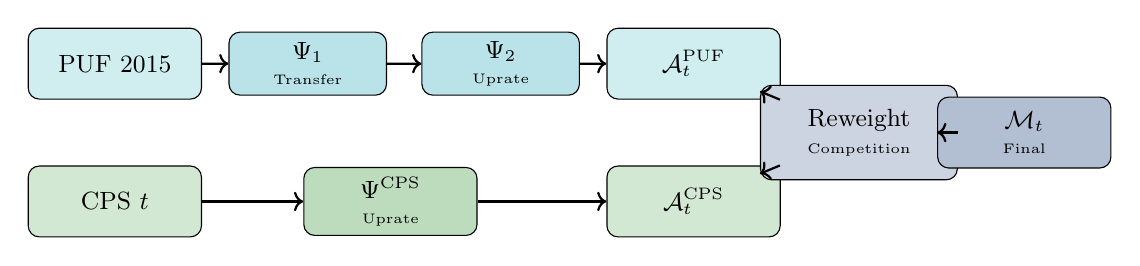
\begin{tikzpicture}[scale=0.7]
    % PUF track
    \node[draw, fill=peteal!20, rounded corners, minimum width=2.2cm, minimum height=0.9cm, align=center]
        (puf0) at (0,2) {\small PUF 2015};
    \node[draw, fill=peteal!30, rounded corners, minimum width=2cm, minimum height=0.8cm, align=center]
        (psi1) at (3.5,2) {\small $\Psi_1$\\[-3pt]\tiny Transfer};
    \node[draw, fill=peteal!30, rounded corners, minimum width=2cm, minimum height=0.8cm, align=center]
        (psi2) at (7,2) {\small $\Psi_2$\\[-3pt]\tiny Uprate};
    \node[draw, fill=peteal!20, rounded corners, minimum width=2.2cm, minimum height=0.9cm, align=center]
        (puft) at (10.5,2) {\small $\mathcal{A}_t^{\text{PUF}}$};

    \draw[->, thick] (puf0) -- (psi1);
    \draw[->, thick] (psi1) -- (psi2);
    \draw[->, thick] (psi2) -- (puft);

    % CPS track
    \node[draw, fill=policygreen!20, rounded corners, minimum width=2.2cm, minimum height=0.9cm, align=center]
        (cps0) at (0,-0.5) {\small CPS $t$};
    \node[draw, fill=policygreen!30, rounded corners, minimum width=2.2cm, minimum height=0.8cm, align=center]
        (psicps) at (5,-0.5) {\small $\Psi^{\text{CPS}}$\\[-3pt]\tiny Uprate};
    \node[draw, fill=policygreen!20, rounded corners, minimum width=2.2cm, minimum height=0.9cm, align=center]
        (cpst) at (10.5,-0.5) {\small $\mathcal{A}_t^{\text{CPS}}$};

    \draw[->, thick] (cps0) -- (psicps);
    \draw[->, thick] (psicps) -- (cpst);

    % Reweighting stage
    \node[draw, fill=taxblue!20, rounded corners, minimum width=2.5cm, minimum height=1.2cm, align=center]
        (reweight) at (13.5,0.75) {\small Reweight\\[-2pt]\tiny Competition};
    \node[draw, fill=taxblue!30, rounded corners, minimum width=2.2cm, minimum height=0.9cm, align=center]
        (final) at (16.5,0.75) {\small $\mathcal{M}_t$\\[-3pt]\tiny Final};

    \draw[->, thick] (puft) -- (reweight);
    \draw[->, thick] (cpst) -- (reweight);
    \draw[->, thick] (reweight) -- (final);
\end{tikzpicture}
\end{center}

\vspace{0.1cm}

\begin{columns}
\begin{column}{0.48\textwidth}
\textbf{PUF Track:} Admin data foundation
\begin{itemize}
    \item $\Psi_1$: Transfer CPS patterns for missing variables \textit{while preserving PUF income}
    \item $\Psi_2$: Uprate 2015 → $t$ via uprating factors 
\end{itemize}

\textbf{CPS Track:} $\Psi^{\text{CPS}}$ Uprate 2023 → $t$ via uprating factors
\end{column}

\begin{column}{0.48\textwidth}
\textbf{Reweighting Competition:}
\begin{itemize}
    \item PUF dominates upper tail (no RPS contamination)
    \item CPS contributes rich demographics
    \item Optimal weights via constrained optimization
\end{itemize}
$$\mathcal{M}_t = \text{Reweight}(\mathcal{A}_t^{\text{PUF}} \cup \mathcal{A}_t^{\text{CPS}})$$
\end{column}
\end{columns}
\end{frame}

\begin{frame}{Dual-Source Competitive Reweighting}

\begin{center}
\textbf{Final Dataset Construction:} $\mathcal{M}_t = \text{Reweight}(\mathcal{A}_t^{\text{PUF}} \cup \mathcal{A}_t^{\text{CPS}})$
\end{center}

\vspace{0.3cm}

\begin{columns}
\begin{column}{0.55\textwidth}
  \textbf{Choose w with Help From the Matrix Equation:}

\vspace{0.2cm}
$$\mathbf{t} = \mathbf{X}\mathbf{w}$$

\vspace{0.2cm}
\begin{itemize}
    \item $\mathbf{t}$: Calibration targets
    \item $\mathbf{X}$: Household characteristics matrix
    \item $\mathbf{w}$: Household weights)
\end{itemize}

\vspace{0.3cm}
\textbf{Calibration Target Categories:}
\begin{itemize}
    \item IRS SOI statistics
    \item Benefit program participation rates
    \item Demographic distributions
\end{itemize}

\end{column}

\begin{column}{0.4\textwidth}
\textbf{Competition Outcome:}

\vspace{0.3cm}

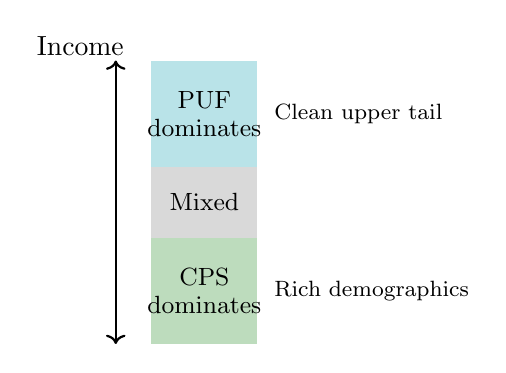
\begin{tikzpicture}[scale=0.9]
    \draw[<->, thick] (0,0) -- (0,4);
    \node at (-0.5,4.2) {Income};

    \fill[policygreen!30] (0.5,0) rectangle (2,1.5);
    \node[align=center] at (1.25,0.75) {\small CPS\\[-2pt]\small dominates};

    \fill[gray!30] (0.5,1.5) rectangle (2,2.5);
    \node[align=center] at (1.25,2) {\small Mixed};

    \fill[peteal!30] (0.5,2.5) rectangle (2,4);
    \node[align=center] at (1.25,3.25) {\small PUF\\[-2pt]\small dominates};

    \node[right, align=left] at (2.1,0.75) {\footnotesize Rich demographics};
    \node[right, align=left] at (2.1,3.25) {\footnotesize Clean upper tail};
\end{tikzpicture}

\end{column}
\end{columns}

\vspace{0.3cm}

\begin{block}{Key Advantage}
Exploits complementary strengths: PUF's unperturbed admin data for high incomes + CPS's comprehensive demographics for broader population
\end{block}

\end{frame}

\section{Sub-National Matrix Optimization}

\begin{frame}{Getting Enough Data For Local Areas: Universal Donor Households}
\framesubtitle{One household, multiple geographies, optimised weights}

\begin{center}
\textbf{Universal donor households}
\vspace{0.3cm}

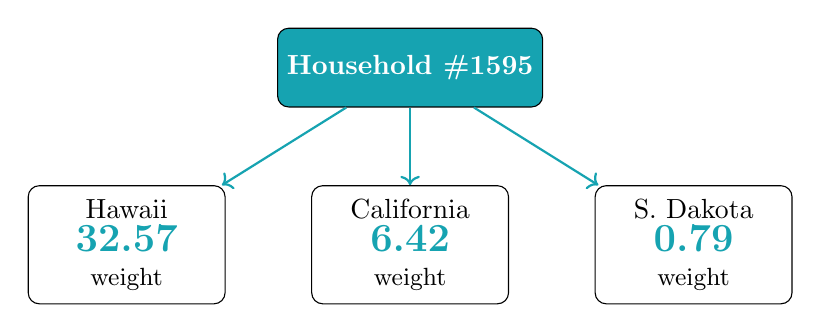
\begin{tikzpicture}[scale=0.9]
    \node[draw, fill=peteal, text=white, rounded corners, font=\bfseries, minimum width=3cm, minimum height=1cm]
        (hh) at (0,0) {Household \#1595};

    \node[draw, fill=white, rounded corners, minimum width=2.5cm, minimum height=1.5cm, align=center]
        (hi) at (-4,-2.5) {Hawaii \\ {\Large \textcolor{peteal}{\textbf{32.57}}} \\ {\small weight}};
    \node[draw, fill=white, rounded corners, minimum width=2.5cm, minimum height=1.5cm, align=center]
        (ca) at (0,-2.5) {California \\ {\Large \textcolor{peteal}{\textbf{6.42}}} \\ {\small weight}};
    \node[draw, fill=white, rounded corners, minimum width=2.5cm, minimum height=1.5cm, align=center]
        (sd) at (4,-2.5) {S. Dakota \\ {\Large \textcolor{peteal}{\textbf{0.79}}} \\ {\small weight}};

    \draw[->, thick, peteal] (hh) -- (hi);
    \draw[->, thick, peteal] (hh) -- (ca);
    \draw[->, thick, peteal] (hh) -- (sd);
\end{tikzpicture}
\end{center}

\end{frame}

\begin{frame}{X for Local Area Stacking is Sparse}

\begin{center}
\small
\renewcommand{\arraystretch}{1.2}
\begin{tabular}{l|cccccc}
& H1\_CA & H2\_CA & H3\_CA & H1\_TX & H2\_TX & H3\_TX \\
\hline
national\_employment & \cellcolor{peteal!30}X & \cellcolor{peteal!30}X & \cellcolor{peteal!30}X & \cellcolor{peteal!30}X & \cellcolor{peteal!30}X & \cellcolor{peteal!30}X \\
national\_tax\_revenue & \cellcolor{peteal!30}X & \cellcolor{peteal!30}X & \cellcolor{peteal!30}X & \cellcolor{peteal!30}X & \cellcolor{peteal!30}X & \cellcolor{peteal!30}X \\
CA\_age\_0\_5 & \cellcolor{peteal!30}X & \cellcolor{peteal!30}X & \cellcolor{peteal!30}X & \cellcolor{gray!30}0 & \cellcolor{gray!30}0 & \cellcolor{gray!30}0 \\
CA\_age\_5\_10 & \cellcolor{peteal!30}X & \cellcolor{peteal!30}X & \cellcolor{peteal!30}X & \cellcolor{gray!30}0 & \cellcolor{gray!30}0 & \cellcolor{gray!30}0 \\
CA\_age\_10\_15 & \cellcolor{peteal!30}X & \cellcolor{peteal!30}X & \cellcolor{peteal!30}X & \cellcolor{gray!30}0 & \cellcolor{gray!30}0 & \cellcolor{gray!30}0 \\
TX\_age\_0\_5 & \cellcolor{gray!30}0 & \cellcolor{gray!30}0 & \cellcolor{gray!30}0 & \cellcolor{peteal!30}X & \cellcolor{peteal!30}X & \cellcolor{peteal!30}X \\
TX\_age\_5\_10 & \cellcolor{gray!30}0 & \cellcolor{gray!30}0 & \cellcolor{gray!30}0 & \cellcolor{peteal!30}X & \cellcolor{peteal!30}X & \cellcolor{peteal!30}X \\
TX\_age\_10\_15 & \cellcolor{gray!30}0 & \cellcolor{gray!30}0 & \cellcolor{gray!30}0 & \cellcolor{peteal!30}X & \cellcolor{peteal!30}X & \cellcolor{peteal!30}X \\
\end{tabular}
\end{center}

\vspace{0.5cm}

\begin{columns}
\begin{column}{0.5\textwidth}
\begin{itemize}
    \item \textbf{X} = household contributes
    \item \textbf{0} = household doesn't contribute
\end{itemize}
\end{column}
\begin{column}{0.5\textwidth}
\begin{itemize}
    \item 99\% sparsity (23 GB → 166 MB) with appropriate structures
    \item Scales to 436 congressional districts
\end{itemize}
\end{column}
\end{columns}

\end{frame}

\begin{frame}{Optional: Enforce Sparsity in Household Weights}
\begin{itemize}
  \item For 10k households by 436 congressional districts is 4.6 million pseudo-households \& weights
  \item For a policy simulator under computational load, it's desireable to have fewer
  \item LASSO will overregularize (push down) wieghts that we want to be large
  \item PolicyEngine has L0- and L2-regularized calibrator based on Louizos et al. 2017
\end{itemize}

\begin{columns}
\begin{column}{0.48\textwidth}
\begin{block}{Sparse X}
{\small \textit{By design}}

\begin{center}
\texttt{\textcolor{peteal}{X X X} \textcolor{gray}{0 0 0}}\\
\texttt{\textcolor{peteal}{X X X} \textcolor{gray}{0 0 0}}\\
\texttt{\textcolor{gray}{0 0 0} \textcolor{peteal}{X X X}}
\end{center}

99\% sparse from geographic constraints
\end{block}
\end{column}

\begin{column}{0.48\textwidth}
\begin{block}{Sparse w}
{\small \textit{Engineered via L0 regularization}}

\begin{center}
\texttt{w\textsubscript{1} = \textcolor{gray}{0.0}}\\
\texttt{w\textsubscript{2} = \textcolor{gray}{0.0}}\\
\texttt{w\textsubscript{3} = \textcolor{peteal}{\textbf{156.7}}}\\
\texttt{w\textsubscript{4} = \textcolor{gray}{0.0}}\\
\texttt{w\textsubscript{5} = \textcolor{peteal}{\textbf{89.3}}}\\
\texttt{w\textsubscript{6} = \textcolor{gray}{0.0}}
\end{center}

Adjustable \% of weights driven to zero
\end{block}
\end{column}
\end{columns}

\end{frame}

\begin{frame}
\begin{center}
\Large{\textbf{Thank You!}}

\vspace{1cm}
\normalsize
Questions and Discussion

\vspace{0.5cm}
Ben.Ogorek@PolicyEngine.org
@BenOgorek on X

\vspace{0.5cm}
\textbf{Resources:}\\
\url{https://policyengine.org}\\
\url{https://github.com/PolicyEngine/policyengine-us-data} \\
\url{https://huggingface.co/policyengine/policyengine-us-data}
\end{center}
\end{frame}

\begin{frame}[allowframebreaks]{References}
  TODO
\bibliography{references}
\end{frame}

\end{document}
